\documentclass[14pt,russian]{scrartcl}
\let\counterwithout\relax
\let\counterwithin\relax
\usepackage{lmodern}
\usepackage{float}
\usepackage{xcolor}
\usepackage{extsizes}
\usepackage{subfig}
\usepackage[export]{adjustbox}
\usepackage{tocvsec2} % возможность менять учитываемую глубину разделов в оглавлении
\usepackage[subfigure]{tocloft}

\usepackage{fancyvrb}
\usepackage{ulem,bm,mathrsfs,ifsym} %зачеркивания, особо жирный стиль и RSFS начертание
\usepackage{sectsty} % переопределение стилей подразделов
%%%%%%%%%%%%%%%%%%%%%%%

%%% Поля и разметка страницы %%%
\usepackage{pdflscape}                              % Для включения альбомных страниц
\usepackage{geometry}                               % Для последующего задания полей
\geometry{a4paper,tmargin=2cm,bmargin=2cm,lmargin=3cm,rmargin=1cm} % тоже самое, но лучше

%%% Математические пакеты %%%
\usepackage{amsthm,amsfonts,amsmath,amssymb,amscd}  % Математические дополнения от AMS
\usepackage{mathtools}                              % Добавляет окружение multlined
\usepackage[perpage]{footmisc}

%%%% Установки для размера шрифта 14 pt %%%%
%% Формирование переменных и констант для сравнения (один раз для всех подключаемых файлов)%%
%% должно располагаться до вызова пакета fontspec или polyglossia, потому что они сбивают его работу
%\newlength{\curtextsize}
%\newlength{\bigtextsize}
%\setlength{\bigtextsize}{13pt}
\KOMAoptions{fontsize=14pt}

\makeatletter
\def\showfontsize{\f@size{} point}
\makeatother

%\makeatletter
%\show\f@size                                       % неплохо для отслеживания, но вызывает стопорение процесса, если документ компилируется без команды  -interaction=nonstopmode 
%\setlength{\curtextsize}{\f@size pt}
%\makeatother

%шрифт times
\usepackage{tempora}

   %%% Решение проблемы копирования текста в буфер кракозябрами
%    \input glyphtounicode.tex
%    \input glyphtounicode-cmr.tex %from pdfx package
%    \pdfgentounicode=1
    \usepackage{cmap}                               % Улучшенный поиск русских слов в полученном pdf-файле
    \usepackage[T2A]{fontenc}                       % Поддержка русских букв
    \usepackage[utf8]{inputenc}                     % Кодировка utf8
    \usepackage[english, main=russian]{babel}            % Языки: русский, английский
%   \IfFileExists{pscyr.sty}{\usepackage{pscyr}}{}  % Красивые русские шрифты
%\renewcommand{\rmdefault}{ftm}
%%% Оформление абзацев %%%
\usepackage{indentfirst}                            % Красная строка
%\usepackage{eskdpz}

%%% Таблицы %%%
\usepackage{longtable}                              % Длинные таблицы
\usepackage{multirow,makecell,array}                % Улучшенное форматирование таблиц
\usepackage{booktabs}                               % Возможность оформления таблиц в классическом книжном стиле (при правильном использовании не противоречит ГОСТ)

%%% Общее форматирование
\usepackage{soulutf8}                               % Поддержка переносоустойчивых подчёркиваний и зачёркиваний
\usepackage{icomma}                                 % Запятая в десятичных дробях



%%% Изображения %%%
\usepackage{graphicx}                               % Подключаем пакет работы с графикой
\usepackage{wrapfig}

%%% Списки %%%
\usepackage{enumitem}

%%% Подписи %%%
\usepackage{caption}                                % Для управления подписями (рисунков и таблиц) % Может управлять номерами рисунков и таблиц с caption %Иногда может управлять заголовками в списках рисунков и таблиц
%% Использование:
%\begin{table}[h!]\ContinuedFloat - чтобы не переключать счетчик
%\captionsetup{labelformat=continued}% должен стоять до самого caption
%\caption{}
% либо ручками \caption*{Продолжение таблицы~\ref{...}.} :)

%%% Интервалы %%%

%%% Счётчики %%%
\usepackage[figure,table,section]{totalcount}               % Счётчик рисунков и таблиц
\DeclareTotalCounter{lstlisting}
\usepackage{totcount}                               % Пакет создания счётчиков на основе последнего номера подсчитываемого элемента (может требовать дважды компилировать документ)
\usepackage{totpages}                               % Счётчик страниц, совместимый с hyperref (ссылается на номер последней страницы). Желательно ставить последним пакетом в преамбуле

%%% Продвинутое управление групповыми ссылками (пока только формулами) %%%
%% Кодировки и шрифты %%%

%   \newfontfamily{\cyrillicfont}{Times New Roman}
%   \newfontfamily{\cyrillicfonttt}{CMU Typewriter Text}
	%\setmainfont{Times New Roman}
	%\newfontfamily\cyrillicfont{Times New Roman}
	%\setsansfont{Times New Roman}                    %% задаёт шрифт без засечек
%	\setmonofont{Liberation Mono}               %% задаёт моноширинный шрифт
 %   \IfFileExists{pscyr.sty}{\renewcommand{\rmdefault}{ftm}}{}
%%% Интервалы %%%
%linespread-реализация ближе к реализации полуторного интервала в ворде.
%setspace реализация заточена под шрифты 10, 11, 12pt, под остальные кегли хуже, но всё же ближе к типографской классике. 
\linespread{1.3}                    % Полуторный интервал (ГОСТ Р 7.0.11-2011, 5.3.6)
%\renewcommand{\@biblabel}[1]{#1}

%%% Гиперссылки %%%
\usepackage{hyperref}

%%% Выравнивание и переносы %%%
\sloppy                             % Избавляемся от переполнений
\clubpenalty=10000                  % Запрещаем разрыв страницы после первой строки абзаца
\widowpenalty=10000                 % Запрещаем разрыв страницы после последней строки абзаца

\makeatletter % малые заглавные, small caps shape
\let\@@scshape=\scshape
\renewcommand{\scshape}{%
  \ifnum\strcmp{\f@series}{bx}=\z@
    \usefont{T1}{cmr}{bx}{sc}%
  \else
    \ifnum\strcmp{\f@shape}{it}=\z@
      \fontshape{scsl}\selectfont
    \else
      \@@scshape
    \fi
  \fi}
\makeatother

%%% Подписи %%%
%\captionsetup{%
%singlelinecheck=off,                % Многострочные подписи, например у таблиц
%skip=2pt,                           % Вертикальная отбивка между подписью и содержимым рисунка или таблицы определяется ключом
%justification=centering,            % Центрирование подписей, заданных командой \caption
%}
%%%        Подключение пакетов                 %%%
\usepackage{ifthen}                 % добавляет ifthenelse
%%% Инициализирование переменных, не трогать!  %%%
\newcounter{intvl}
\newcounter{otstup}
\newcounter{contnumeq}
\newcounter{contnumfig}
\newcounter{contnumtab}
\newcounter{pgnum}
\newcounter{bibliosel}
\newcounter{chapstyle}
\newcounter{headingdelim}
\newcounter{headingalign}
\newcounter{headingsize}
\newcounter{tabcap}
\newcounter{tablaba}
\newcounter{tabtita}
%%%%%%%%%%%%%%%%%%%%%%%%%%%%%%%%%%%%%%%%%%%%%%%%%%

%%% Область упрощённого управления оформлением %%%

%% Интервал между заголовками и между заголовком и текстом
% Заголовки отделяют от текста сверху и снизу тремя интервалами (ГОСТ Р 7.0.11-2011, 5.3.5)
\setcounter{intvl}{3}               % Коэффициент кратности к размеру шрифта

%% Отступы у заголовков в тексте
\setcounter{otstup}{0}              % 0 --- без отступа; 1 --- абзацный отступ

%% Нумерация формул, таблиц и рисунков
\setcounter{contnumeq}{1}           % Нумерация формул: 0 --- пораздельно (во введении подряд, без номера раздела); 1 --- сквозная нумерация по всей диссертации
\setcounter{contnumfig}{1}          % Нумерация рисунков: 0 --- пораздельно (во введении подряд, без номера раздела); 1 --- сквозная нумерация по всей диссертации
\setcounter{contnumtab}{1}          % Нумерация таблиц: 0 --- пораздельно (во введении подряд, без номера раздела); 1 --- сквозная нумерация по всей диссертации

%% Оглавление
\setcounter{pgnum}{0}               % 0 --- номера страниц никак не обозначены; 1 --- Стр. над номерами страниц (дважды компилировать после изменения)

%% Библиография
\setcounter{bibliosel}{1}           % 0 --- встроенная реализация с загрузкой файла через движок bibtex8; 1 --- реализация пакетом biblatex через движок biber

%% Текст и форматирование заголовков
\setcounter{chapstyle}{1}           % 0 --- разделы только под номером; 1 --- разделы с названием "Глава" перед номером
\setcounter{headingdelim}{1}        % 0 --- номер отделен пропуском в 1em или \quad; 1 --- номера разделов и приложений отделены точкой с пробелом, подразделы пропуском без точки; 2 --- номера разделов, подразделов и приложений отделены точкой с пробелом.

%% Выравнивание заголовков в тексте
\setcounter{headingalign}{0}        % 0 --- по центру; 1 --- по левому краю

%% Размеры заголовков в тексте
\setcounter{headingsize}{0}         % 0 --- по ГОСТ, все всегда 14 пт; 1 --- пропорционально изменяющийся размер в зависимости от базового шрифта

%% Подпись таблиц
\setcounter{tabcap}{0}              % 0 --- по ГОСТ, номер таблицы и название разделены тире, выровнены по левому краю, при необходимости на нескольких строках; 1 --- подпись таблицы не по ГОСТ, на двух и более строках, дальнейшие настройки: 
%Выравнивание первой строки, с подписью и номером
\setcounter{tablaba}{2}             % 0 --- по левому краю; 1 --- по центру; 2 --- по правому краю
%Выравнивание строк с самим названием таблицы
\setcounter{tabtita}{1}             % 0 --- по левому краю; 1 --- по центру; 2 --- по правому краю

%%% Рисунки %%%
\DeclareCaptionLabelSeparator*{emdash}{~--- }             % (ГОСТ 2.105, 4.3.1)
\captionsetup[figure]{labelsep=emdash,font=onehalfspacing,position=bottom}

%%% Таблицы %%%
\ifthenelse{\equal{\thetabcap}{0}}{%
    \newcommand{\tabcapalign}{\raggedright}  % по левому краю страницы или аналога parbox
}

\ifthenelse{\equal{\thetablaba}{0} \AND \equal{\thetabcap}{1}}{%
    \newcommand{\tabcapalign}{\raggedright}  % по левому краю страницы или аналога parbox
}

\ifthenelse{\equal{\thetablaba}{1} \AND \equal{\thetabcap}{1}}{%
    \newcommand{\tabcapalign}{\centering}    % по центру страницы или аналога parbox
}

\ifthenelse{\equal{\thetablaba}{2} \AND \equal{\thetabcap}{1}}{%
    \newcommand{\tabcapalign}{\raggedleft}   % по правому краю страницы или аналога parbox
}

\ifthenelse{\equal{\thetabtita}{0} \AND \equal{\thetabcap}{1}}{%
    \newcommand{\tabtitalign}{\raggedright}  % по левому краю страницы или аналога parbox
}

\ifthenelse{\equal{\thetabtita}{1} \AND \equal{\thetabcap}{1}}{%
    \newcommand{\tabtitalign}{\centering}    % по центру страницы или аналога parbox
}

\ifthenelse{\equal{\thetabtita}{2} \AND \equal{\thetabcap}{1}}{%
    \newcommand{\tabtitalign}{\raggedleft}   % по правому краю страницы или аналога parbox
}

\DeclareCaptionFormat{tablenocaption}{\tabcapalign #1\strut}        % Наименование таблицы отсутствует
\ifthenelse{\equal{\thetabcap}{0}}{%
    \DeclareCaptionFormat{tablecaption}{\tabcapalign #1#2#3}
    \captionsetup[table]{labelsep=emdash}                       % тире как разделитель идентификатора с номером от наименования
}{%
    \DeclareCaptionFormat{tablecaption}{\tabcapalign #1#2\par%  % Идентификатор таблицы на отдельной строке
        \tabtitalign{#3}}                                       % Наименование таблицы строкой ниже
    \captionsetup[table]{labelsep=space}                        % пробельный разделитель идентификатора с номером от наименования
}

\DeclareCaptionFormat{listings}{%
%\setlength{\fboxsep}{0pt}%
\parbox[top][0pt][l]{\textwidth}{\hspace{0pt}#1#2#3}}

\captionsetup[lstlisting]{justification=raggedright, singlelinecheck=off}

\captionsetup[table]{format=tablecaption,singlelinecheck=off,font=onehalfspacing,position=top,skip=-5pt, justification=raggedright}

\captionsetup[tabular]{format=tablecaption,singlelinecheck=off,font=onehalfspacing,position=top,skip=-5pt, justification=raggedright}

\DeclareCaptionLabelFormat{continued}{Продолжение таблицы~#2}
\setlength{\belowcaptionskip}{.2cm}
\setlength{\intextsep}{0ex}

%%% Подписи подрисунков %%%
\renewcommand{\thesubfigure}{\asbuk{subfigure}}           % Буквенные номера подрисунков
\captionsetup[subfigure]{font={normalsize},               % Шрифт подписи названий подрисунков (не отличается от основного)
    labelformat=brace,                                    % Формат обозначения подрисунка
    justification=centering,                              % Выключка подписей (форматирование), один из вариантов            
}
%\DeclareCaptionFont{font12pt}{\fontsize{12pt}{13pt}\selectfont} % объявляем шрифт 12pt для использования в подписях, тут же надо интерлиньяж объявлять, если не наследуется
%\captionsetup[subfigure]{font={font12pt}}                 % Шрифт подписи названий подрисунков (всегда 12pt)

%%% Настройки гиперссылок %%%

\definecolor{linkcolor}{rgb}{0.0,0,0}
\definecolor{citecolor}{rgb}{0,0.0,0}
\definecolor{urlcolor}{rgb}{0,0,0}

\hypersetup{
    linktocpage=true,           % ссылки с номера страницы в оглавлении, списке таблиц и списке рисунков
%    linktoc=all,                % both the section and page part are links
%    pdfpagelabels=false,        % set PDF page labels (true|false)
    plainpages=true,           % Forces page anchors to be named by the Arabic form  of the page number, rather than the formatted form
    colorlinks,                 % ссылки отображаются раскрашенным текстом, а не раскрашенным прямоугольником, вокруг текста
    linkcolor={linkcolor},      % цвет ссылок типа ref, eqref и подобных
    citecolor={citecolor},      % цвет ссылок-цитат
    urlcolor={urlcolor},        % цвет гиперссылок
    pdflang={ru},
}
\urlstyle{same}
%%% Шаблон %%%
%\DeclareRobustCommand{\todo}{\textcolor{red}}       % решаем проблему превращения названия цвета в результате \MakeUppercase, http://tex.stackexchange.com/a/187930/79756 , \DeclareRobustCommand protects \todo from expanding inside \MakeUppercase
\setlength{\parindent}{2.5em}                       % Абзацный отступ. Должен быть одинаковым по всему тексту и равен пяти знакам (ГОСТ Р 7.0.11-2011, 5.3.7).

%%% Списки %%%
% Используем дефис для ненумерованных списков (ГОСТ 2.105-95, 4.1.7)
%\renewcommand{\labelitemi}{\normalfont\bfseries~{---}} 
\renewcommand{\labelitemi}{\bfseries~{---}} 
\setlist{nosep,%                                    % Единый стиль для всех списков (пакет enumitem), без дополнительных интервалов.
    labelindent=\parindent,leftmargin=*%            % Каждый пункт, подпункт и перечисление записывают с абзацного отступа (ГОСТ 2.105-95, 4.1.8)
}
%%%%%%%%%%%%%%%%%%%%%%
%\usepackage{xltxtra} % load xunicode

\usepackage{ragged2e}
\usepackage[explicit]{titlesec}
\usepackage{placeins}
\usepackage{xparse}

\usepackage{listingsutf8}
\usepackage{url} %пакеты расширений
\usepackage{algorithm, algorithmicx}
\usepackage[noend]{algpseudocode}
\usepackage{blkarray}
\usepackage{chngcntr}
\usepackage{tabularx}
\newcommand*\template[1]{\text{<}#1\text{>}}

  
\titleformat{name=\section,numberless}[block]{\normalfont\Large\centering}{}{0em}{#1}
\titleformat{\section}[block]{\normalfont\Large\bfseries\raggedright}{}{0em}{\thesection\hspace{0.25em}#1}
\titleformat{\subsection}[block]{\normalfont\Large\bfseries\raggedright}{}{0em}{\thesubsection\hspace{0.25em}#1}
\titleformat{\subsubsection}[block]{\normalfont\large\bfseries\raggedright}{}{0em}{\thesubsubsection\hspace{0.25em}#1}

\let\Algorithm\algorithm
\renewcommand\algorithm[1][]{\Algorithm[#1]\setstretch{1.5}}

\usepackage{relsize}
\usepackage{pifont}
\usepackage{calc}
\usepackage{suffix}
\usepackage{csquotes}
\DeclareQuoteStyle{russian}
    {\guillemotleft}{\guillemotright}[0.025em]
    {\quotedblbase}{\textquotedblleft}
\ExecuteQuoteOptions{style=russian}
\newcommand{\enq}[1]{\enquote{#1}}  
\newcommand{\eng}[1]{\begin{english}#1\end{english}}
% Подчиненные счетчики в окружениях http://old.kpfu.ru/journals/izv_vuz/arch/sample1251.tex
\newcounter{cTheorem} 
\newcounter{cDefinition}
\newcounter{cConsequent}
\newcounter{cExample}
\newcounter{cLemma}
\newcounter{cConjecture}
\newtheorem{Theorem}{Теорема}[cTheorem]
\newtheorem{Definition}{Определение}[cDefinition]
\newtheorem{Consequent}{Следствие}[cConsequent]
\newtheorem{Example}{Пример}[cExample]
\newtheorem{Lemma}{Лемма}[cLemma]
\newtheorem{Conjecture}{Гипотеза}[cConjecture]

\renewcommand{\theTheorem}{\arabic{Theorem}}
\renewcommand{\theDefinition}{\arabic{Definition}}
\renewcommand{\theConsequent}{\arabic{Consequent}}
\renewcommand{\theExample}{\arabic{Example}}
\renewcommand{\theLemma}{\arabic{Lemma}}
\renewcommand{\theConjecture}{\arabic{Conjecture}}
%\makeatletter
\NewDocumentCommand{\Newline}{}{\text{\\}}
\newcommand{\sequence}[2]{\ensuremath \left(#1,\ \dots,\ #2\right)}

\definecolor{mygreen}{rgb}{0,0.6,0}
\definecolor{mygray}{rgb}{0.5,0.5,0.5}
\definecolor{mymauve}{rgb}{0.58,0,0.82}
\renewcommand{\listalgorithmname}{Список алгоритмов}
\floatname{algorithm}{Листинг}
\renewcommand{\lstlistingname}{Листинг}
\renewcommand{\thealgorithm}{\arabic{algorithm}}

\newcommand{\refAlgo}[1]{(листинг \ref{#1})}
\newcommand{\refImage}[1]{(рисунок \ref{#1})}

\renewcommand{\theenumi}{\arabic{enumi}.}% Меняем везде перечисления на цифра.цифра	
\renewcommand{\labelenumi}{\arabic{enumi}.}% Меняем везде перечисления на цифра.цифра
\renewcommand{\theenumii}{\arabic{enumii}}% Меняем везде перечисления на цифра.цифра
\renewcommand{\labelenumii}{(\arabic{enumii})}% Меняем везде перечисления на цифра.цифра
\renewcommand{\theenumiii}{\roman{enumiii}}% Меняем везде перечисления на цифра.цифра
\renewcommand{\labelenumiii}{(\roman{enumiii})}% Меняем везде перечисления на цифра.цифра
%\newfontfamily\AnkaCoder[Path=src/fonts/]{AnkaCoder-r.ttf}
\renewcommand{\labelitemi}{---}
\renewcommand{\labelitemii}{---}

%\usepackage{courier}

\graphicspath{ {./img/} }

\lstdefinelanguage{Refal}{
  alsodigit = {.,<,>},
  morekeywords = [1]{$ENTRY},
  morekeywords = [2]{Go, Put, Get, Open, Close, Arg, Add, Sub, Mul, Div, Symb, Explode, Implode},
  %keyword4
  morekeywords = [3]{<,>},
  %keyword5
  morekeywords = [4]{e.,t.,s.},
  sensitive = true,
  morecomment = [l]{*},
  morecomment = [s]{/*}{*/},
  commentstyle = \color{mygreen},
  morestring = [b]",
  morestring = [b]',
  stringstyle = \color{purple}
}

\makeatletter
\def\p@subsection{}
\def\p@subsubsection{\thesection\,\thesubsection\,}
\makeatother
\newcommand{\prog}[1]{{\ttfamily\small#1}}
\lstset{ %
  backgroundcolor=\color{white},   % choose the background color; you must add \usepackage{color} or \usepackage{xcolor}
  basicstyle=\ttfamily\footnotesize, 
  %basicstyle=\footnotesize\AnkaCoder,        % the size of the fonts that are used for the code
  breakatwhitespace=false,         % sets if automatic breaks shoulbd only happen at whitespace
  breaklines=true,                 % sets automatic line breaking
  captionpos=top,                    % sets the caption-position to bottom
  commentstyle=\color{mygreen},    % comment style
  deletekeywords={...},            % if you want to delete keywords from the given language
  escapeinside={\%*}{*)},          % if you want to add LaTeX within your code
  extendedchars=true,              % lets you use non-ASCII characters; for 8-bits encodings only, does not work with UTF-8
  inputencoding=utf8,
  frame=single,                    % adds a frame around the code
  keepspaces=true,                 % keeps spaces in text, useful for keeping indentation of code (possibly needs columns=flexible)
  keywordstyle=\bf,       % keyword style
  language=Refal,                    % the language of the code
  morekeywords={<,>,$ENTRY,Go,Arg, Open, Close, e., s., t., Get, Put}, 
  							       % if you want to add more keywords to the set
  numbers=left,                    % where to put the line-numbers; possible values are (none, left, right)
  numbersep=5pt,                   % how far the line-numbers are from the code
  xleftmargin=25pt,
  xrightmargin=25pt,
  numberstyle=\small\color{black}, % the style that is used for the line-numbers
  rulecolor=\color{black},         % if not set, the frame-color may be changed on line-breaks within not-black text (e.g. comments (green here))
  showspaces=false,                % show spaces everywhere adding particular underscores; it overrides 'showstringspaces'
  showstringspaces=false,          % underline spaces within strings only
  showtabs=false,                  % show tabs within strings adding particular underscores
  stepnumber=1,                    % the step between two line-numbers. If it's 1, each line will be numbered
  stringstyle=\color{mymauve},     % string literal style
  tabsize=4,                       % sets default tabsize to 8 spaces
  title=\lstname                   % show the filename of files included with \lstinputlisting; also try caption instead of title
}
\newcommand{\anonsection}[1]{\cleardoublepage
\phantomsection
\addcontentsline{toc}{section}{\protect\numberline{}#1}
\section*{#1}\vspace*{2.5ex} % По госту положены 3 пустые строки после заголовка ненумеруемого раздела
}
\newcommand{\sectionbreak}{\clearpage}
\renewcommand{\sectionfont}{\normalsize} % Сбиваем стиль оглавления в стандартный
\renewcommand{\cftsecleader}{\cftdotfill{\cftdotsep}} % Точки в оглавлении напротив разделов

\renewcommand{\cftsecfont}{\normalfont\large} % Переключение на times в содержании
\renewcommand{\cftsubsecfont}{\normalfont\large} % Переключение на times в содержании

\usepackage{caption} 
%\captionsetup[table]{justification=raggedleft} 
%\captionsetup[figure]{justification=centering,labelsep=endash}
\usepackage{amsmath}    % \bar    (матрицы и проч. ...)
\usepackage{amsfonts}   % \mathbb (символ для множества действительных чисел и проч. ...)
\usepackage{mathtools}  % \abs, \norm
    \DeclarePairedDelimiter\abs{\lvert}{\rvert} % операция модуля
    \DeclarePairedDelimiter\norm{\lVert}{\rVert} % операция нормы
\DeclareTextCommandDefault{\textvisiblespace}{%
  \mbox{\kern.06em\vrule \@height.3ex}%
  \vbox{\hrule \@width.3em}%
  \hbox{\vrule \@height.3ex}}    
\newsavebox{\spacebox}
\begin{lrbox}{\spacebox}
\verb*! !
\end{lrbox}
\newcommand{\aspace}{\usebox{\spacebox}}


\title{Lab 02 report}
\author{Kirill}

\date{\today}

\begin{document}
\thispagestyle{empty}

\noindent \begin{minipage}{0.15\textwidth}
	
\includegraphics[width=\linewidth]{b_logo}
\end{minipage}
\noindent\begin{minipage}{0.85\textwidth}\centering
	\textbf{Министерство науки и высшего образования Российской Федерации}\\
	\textbf{Федеральное государственное бюджетное образовательное учреждение высшего образования}\\
	\textbf{«Московский государственный технический университет имени Н.Э.~Баумана}\\
	\textbf{(национальный исследовательский университет)»}\\
	\textbf{(МГТУ им. Н.Э.~Баумана)}
\end{minipage}

\noindent\rule{16cm}{3pt}
\newline\newline
\noindent ФАКУЛЬТЕТ $\underline{\text{«Информатика и системы управления»}}$ \newline\newline
\noindent КАФЕДРА $\underline{\text{«Программное обеспечение ЭВМ и информационные технологии»}}$\newline


\begin{center}
	\noindent\begin{minipage}{1.3\textwidth}\centering
	\Large\textbf{   ~~~ Лабораторная работа №2}\newline
	\textbf{по дисциплине "Анализ Алгоритмов"}\newline\newline\newline
	\end{minipage}
\end{center}

\noindent\textbf{Тема} $\underline{\text{Умножение матриц}}$\newline\newline
\noindent\textbf{Студент} $\underline{\text{Рядинский К. В.}}$\newline\newline
\noindent\textbf{Группа} $\underline{\text{ИУ7-53Б}}$\newline\newline
\noindent\textbf{Преподаватель} $\underline{\text{Волкова Л. Л.}}$\newline

\begin{center}
	\mbox{}
	\vfill
	Москва
\end{center}

\begin{center}
	\the\year ~г.
\end{center}
\clearpage

\renewcommand\contentsname{\hfill{\normalfont{СОДЕРЖАНИЕ}}\hfill}  %Оглавление
\tableofcontents
\newpage

\anonsection{Введение}

Алгоритм Копперсмита - Винограда --- алгоритм умножение квадратных матриц, предложенный в 1987 году Д. Копперсмитом и Ш. Виноградом. В исходной версии асимптотическая сложность алгоритма составляла $O(n^{2.3755})$, где $n$ --- размер стороны матрицы. Алгоритм Копперсмита -- Винограда, с учетом серии улучшений и доработок в последующие годы, обладает лучшей асимптотикой среди известных алгоритмов умножения матриц.


Алгоритм Штрассена предназначен для быстрого умножения матриц. Он был разработан Фолькером Штрассеном в 1969 году и является обобщением метода умножения Карацубы на матрицы.

В отличие от традиционного алгоритма множения матриц, алгоритм Штрассена умножает матрицы за время $\Theta(n^{\log_2{7}}) = O(n^{2.81})$

Несмотря на то, что алгоритм Штрассена является асимптотически не самым быстрым из существующих алгоритмов быстрого умножения матриц, он проще программируется и эффективнее при умножении матриц относительно малого размера.

Задачи лабораторной работы:

\begin{itemize}
    \item рассчитать трудоемкость алгоритмов умножения матриц;
    \item реализовать классический алгоритм умножения матриц;
    \item реализовать алгоритм Копперсмита — Винограда;
    \item реализовать улучшенный Алгоритм Копперсмита -- Винограда;
    \item сравнить их временные характеристики экспериментально;
    \item на основании проделанной работы сделать выводы.
\end{itemize}

\section{Аналитическая часть}

В данном разделе будут рассмотрены алгоритмы умножения матриц

\subsection{Стандартный алгоритм}

Пусть даны две прямоугольные матрицы

\begin{equation}
    A =
      \begin{pmatrix}
        a_{11} & a_{12} & \cdots & a_{1m} \\
        a_{21} & a_{22} & \cdots & a_{2m} \\
        \vdots & \vdots & \ddots & \vdots \\
        a_{l1} & a_{l2} & \cdots & a_{lm}
      \end{pmatrix},
\end{equation}

\begin{equation}
    B =
    \begin{pmatrix}
      b_{11} & b_{12} & \cdots & b_{1n} \\
      b_{21} & b_{22} & \cdots & b_{2n} \\
      \vdots & \vdots & \ddots & \vdots \\
      b_{m1} & b_{m2} & \cdots & b_{mn}
    \end{pmatrix}.
\end{equation}

Тогда матрица $C$ размерностью $l \times n$

\begin{equation}
    C =
      \begin{pmatrix}
        c_{11} & c_{12} & \cdots & c_{1n} \\
        c_{21} & c_{22} & \cdots & c_{2n} \\
        \vdots & \vdots & \ddots & \vdots \\
        c_{l1} & c_{l2} & \cdots & c_{ln}
      \end{pmatrix},
\end{equation}

в которой:

\begin{equation}
    \displaystyle
    c_{ij} = \displaystyle\sum_{r = 1}^{m} a_{ir} b_{rj}, \quad (i = \overline{1, l}; j = \overline{1, n} )
\end{equation}

будет называться произведением матриц $A$ и $B$. Стандартный алгоритм
реализует данную формулу.

\subsection{Алгоритм Копперсмита -- Винограда}

В результате умножения двух матриц, каждый элемент в нем представляет собой скалярное произведение соответствующих строки и столбца исходных матриц. Можно заметить, что такое умножение допускает предварительную обработку, позволяющую часть работы выполнить заранее.

Рассмотрим два вектора $V = (v_1, v_2, v_3, v_4)$ и $W = (w_1, w_2, w_3, w_4)$. Их скалярное произведение равно: $V \cdot W = v_1 w_1 + \cdots + v_4 w_4$, что эквивалентно

\begin{equation}
    V \cdot W = (v_1 + w_1)(v_2 + w_1) + (v_3 + w_4)(v_4 + w_3) - v_1 v_2 - v_3 v_4 - w_1 w_2 - w_3 w_4.
\end{equation}

Несмотря на то, что второе выражение требует вычисления большего коли- чества операций, чем стандартный алгоритм: вместо четырех умножений - шесть, а вместо трех сложений - десять, выражение в правой части последнего равенства допускает предварительную обработку: его части можно вычислить заранее и за- помнить для каждой строки первой матрицы и для каждого столбца второй, то для каждого элемента будет необходимо выполнить лишь первые два умножения и последующие пять сложений, а также дополнительно два сложения. Из-за того, что операция сложения быстрее операции умножения, алгоритм должен работать быстрее стандартного.
\subsection{Оптимизированный алгоритм Копперсмита -- Винограда}

В данный алгоритм является оптимизированной версией алгоритма Копперсмита -- Винограда. Следующие выражения были оптимизированы:

\begin{enumerate}
    \item Убраны деления в цикле.
    \item Замена выражения $a = a + \cdots$ на $a += \cdots$.
    \item Шаг в цикле был увеличен на 2.
    \item Добавлен кэш во внутреннем цикле.
\end{enumerate}


\subsection{Вывод}

Были рассмотрены алгоритмы классического умножения матриц и алгоритм Винограда, основное отличие которых — наличие предварительной обработки, а также количество операций умножения.

\section{Конструкторская часть}

В данном разделе будут рассмотрены требования к программному обеспечению, трудоемкость алгоритмов, схемы алгоритмов.

\subsection{Требования к программному обеспечению}

К программе предъявляется ряд требований:
\begin{itemize}
    \item на вход подаются размеры матриц (натуральные числа) и самы матрицы, которые нужно перемножить;
    \item на вход подаются только квадратные матрицы;
    \item на выходе — результаты умножения матриц алгоритмами простого умножения матриц, умножения матриц по Копперсмиту–Винограду и улучшенного умножения матриц по Копперсмиту–Винограду.
\end{itemize}


\subsection{Разработка алгоритмов}

На рисунках \ref{img:canon}-\ref{img:vinograd_opt} приведены схемы алгоритмов простого умножения матриц, умножения матриц по Копперсмиту–Винограду и улучшенного умножения матриц по Копперсмиту–Винограду соответственно.

Для алгоритма Винограда худшим случаем являются матрицы с нечётным общим размером, а лучшим - с чётным, так как отпадает необходимость в последнем цикле.

Данный алгоритм можно оптимизировать:

\begin{enumerate}
    \item Убрать деления в цикле.
    \item Замена выражения $a = a + \cdots $ на $a += \cdots$.
    \item Увеличить шаг в цикле до 2.
    \item Добавлен кэш во внутреннем цикле тройного цикла.
\end{enumerate}

\subsection{Трудоемкость алгоритмов}

Для последующего вычисления трудоемкости необходимо ввести модель вычислений [1].
Трудоемкость алгоритмов будет вычислена по схемам алгоритмов.

\begin{enumerate}
    \item $+, -, /, \%, =, \neq, <, >, \leq, \geq, [ ], *$ ~---~ трудоемкость 1.
    \item Трудоемкость оператора выбора \textit{if} условие \textit{then A else B} рассчитывается, как:

    \begin{equation}
        f_{if} = f_{\text{условия}} + \begin{cases}
                                f_A & \quad \text{если условие выполняется,} \\
                                f_B & \quad \text{иначе}.
                                \end{cases}
    \end{equation}

    \item Трудоемкость цикла расчитывается, как:
    \begin{equation}
        f_{for} = f_{\text{инициализации}} + f_{\text{сравнения}} + N(f_{\text{тела}} + f_{\text{инициализации}} + f_{\text{сравнения}}).
    \end{equation}

    \item Трудоемкость вызова функции равна 0.
\end{enumerate}

\subsubsection{Классический алгоритм}

Трудоемкость классического алгоритма:

$10MNQ + 4MQ + 4M + 2$

\subsubsection{Алгоритм Винограда}

Трудоемкость алгоритма Винограда:

Первый цикл: $\frac{15}{2} \cdot MN + 5 \cdot M + 2$

Второй цикл: $\frac{15}{2} \cdot MN + 5 \cdot M + 2$

Третий цикл: $13 \cdot MNQ + 12 \cdot MQ + 4 \cdot M + 2$

Условный переход:

\begin{equation*}
    \begin{cases}
        2 & \quad \text{,если размер матрицы нечетный} \\
        15 \cdot QM + 4 \cdot M + 2 & \quad \text{,иначе}
    \end{cases}
\end{equation*}

Итого:

\begin{multline*}
    \frac{15}{2} \cdot MN + 5 M + 2 + \frac{15}{2} \cdot MN + 5 M + 2 + 13 MNQ + \\
     + 12 MQ + 4M + 2 + \begin{cases}
        2 & \quad \text{,если размер матрицы нечетный} \\
        15 \cdot MQ + 4M + 2 & \quad \text{,иначе.}
    \end{cases}
\end{multline*}

\subsection{Оптимизированный алгоритм Винограда}

Рассмотрим трудоемкость оптимизированного алгоритма Винограда:

\noindent
Первый цикл: $\frac{11}{2} \cdot MN + 4M + 2$ \\
Второй цикл: $\frac{11}{2} \cdot MN + 4M + 2$ \\
Третий цикл: $\frac{15}{2} \cdot MNQ + 9MQ + 4M + 2$ \\

\noindent
Условный переход: $ \begin{cases}
    1 & \quad \text{, если размер матрицы нечетный} \\
    10 MQ + 4M + 2 & \quad \text{, иначе.}
\end{cases} $

\noindent
Итого: $\frac{11}{2} \cdot MN + 4M + 2 + \frac{11}{2}MN + 4M + 2 + \frac{15}{2}MNQ + 9 MQ + 4M + 2 + \begin{cases}
    1 & \quad \text{, если размер матрицы нечетный} \\
    10 MQ + 4M + 2 & \quad \text{, иначе.}
\end{cases}$

\subsection{Вывод} 

На основе теоретических данных, полученных из аналитического раздела, были построены схемы требуемых алгоритмов и проведена теоретическая оценка трудоемкости.

\begin{figure}
    \centering
    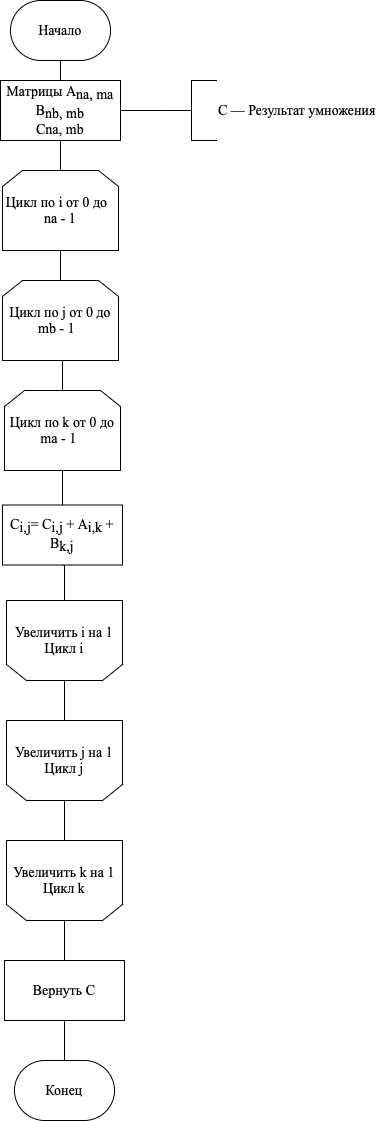
\includegraphics[scale=0.6]{canon.png}
    \caption{Схема алгоритма простого умножения матриц}
    \label{img:canon}
\end{figure}

\begin{figure}
    \centering
    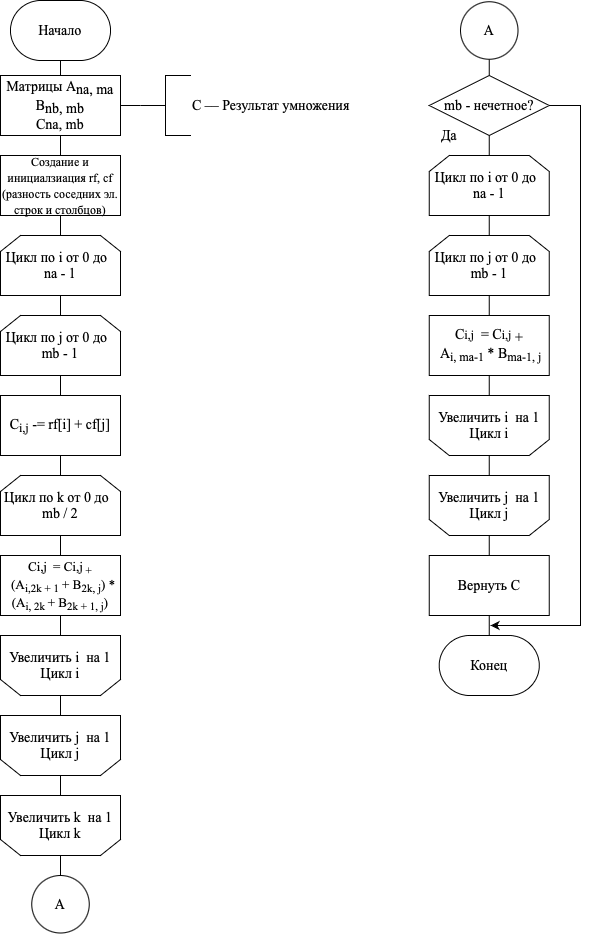
\includegraphics[scale=0.75]{vinograd.png}
    \caption{Схема алгоритма Винограда умножения матриц}
    \label{img:vinograd}
\end{figure}

\begin{figure}
    \centering
    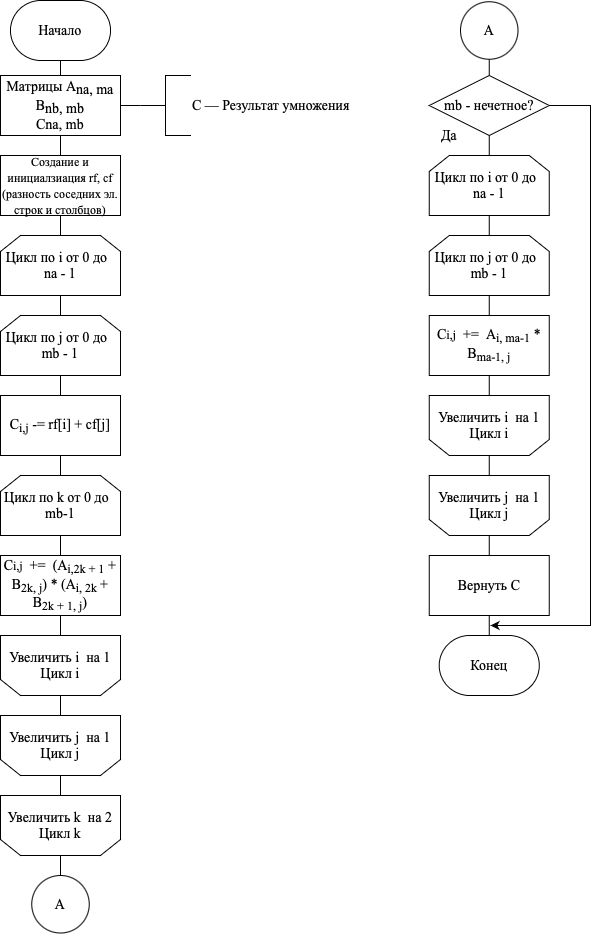
\includegraphics[scale=0.75]{vinograd_opt.png}
    \caption{Схема оптимизированного алгоритма Винограда умножения матриц}
    \label{img:vinograd_opt}
\end{figure}

\section{Технологическая часть}

В данном разделе приведены средства реализации и листинги кода.

\subsection{Средства реализации}


Для реализации программ был выбран язык программирования Rust [2], так как этот язык предоставляет как низкоуровневые интерфейсы, так и высокоуровневые, этот язык безопасен при работе с памятью. Также данный язык был выбран потому, что в нем присутствует инструментарий для замера процессорного времени и тестирования.

\subsection{Листинги кода}

\begin{lstlisting}[caption=Алгоритм простого умножения матриц, label=list:canon, language={}]
pub fn default_mult(m1 : & Matrix<T>, m2 : & Matrix<T>) -> Result<Matrix<T>, &'static str> {
    if m1.col != m2.rows {
        return Err("The number of columns must be equal to number of rows");
    }
    let mut out = Matrix::new_zero(m1.rows, m2.col);
    for i in 0..m1.rows {
        for j in 0..m2.col {
            for k in 0..m1.col {
                out[[i, j]] += m1[[i, k]] * m2[[k, j]];
            }
        }
    }
    Ok(out)
}
\end{lstlisting}

\begin{lstlisting}[caption=Алгоритм умножения матриц Винограда, label=list:vinograd, language={}]
pub fn vinograd_mult(m1 : & Matrix<T>, m2 : & Matrix<T>) -> Result<Matrix<T>, &'static str> {
    if m1.rows != m1.col || m2.col != m2.rows || m1.col != m2.col {
        return Err("Matrices must be square and have equal size");
    }

    let mut out : Matrix<T> = Matrix::new_zero(m1.rows, m2.col);

    let mut row_factor : Vec<T> = vec![Default::default(); m1.rows];
    let mut col_factor : Vec<T> = vec![Default::default(); m2.col];

    for i in 0..m1.rows {
        for j in 0..m1.col / 2 {
            row_factor[i] += m1[[i, j * 2]] * m1[[i, j * 2 + 1]]
        }
    }

    for i in 0..m2.col {
        for j in 0..m2.rows / 2 {
            col_factor[i] += m2[[j * 2, i]] * m2[[j * 2 + 1, i]]
        }
    }

    for i in 0..m1.rows {
        for j in 0..m2.col {
            out[[i, j]] -= row_factor[i] + col_factor[j];

            for k in 0..m1.col / 2 {
                out[[i, j]] += (m1[[i, 2 * k + 1]] + m2[[2 * k, j]]) * (m1[[i, 2 * k]] + m2[[2 * k + 1, j]]);
            }
        }
    }

    if m1.col % 2 > 0{
        for i in 0..m1.rows {
            for j in 0..m2.col {
                out[[i, j]] += m1[[i, m1.col - 1]] * m2[[m1.col - 1, j]];
            }
        }
    }

    Ok(out)
}
\end{lstlisting}

\begin{lstlisting}[caption=Оптимизированный алгоритм умножения матриц Винограда, label=list:vinograd, language={}]
pub fn vinograd_opt_mult(m1 : & Matrix<T>, m2 : & Matrix<T>) -> Result<Matrix<T>, &'static str> {
    if m1.rows != m1.col || m2.col != m2.rows || m1.col != m2.col {
        return Err("Matrices must be square and have equal size");
    }

    let mut out : Matrix<T> = Matrix::new_zero(m1.rows, m2.col);

    let mut row_factor : Vec<T> = vec![Default::default(); m1.rows];
    let mut col_factor : Vec<T> = vec![Default::default(); m2.col];

    let m1_col_mod = m1.col % 2;
    let m2_row_mod = m2.rows % 2;

    for i in 0..m1.rows {
        for j in (0..m1.col - m1_col_mod).step_by(2) {
            row_factor[i] += m1[[i, j]] * m1[[i, j + 1]]
        }
    }

    for i in 0..m2.col {
        for j in (0..m2.rows - m2_row_mod).step_by(2) {
            col_factor[i] += m2[[j, i]] * m2[[j + 1, i]]
        }
    }

    for i in 0..m1.rows {
        for j in 0..m2.col {
            let mut buf : T = -(row_factor[i] + col_factor[j]);

            for k in (0..m1.col - m1_col_mod).step_by(2) {
                buf += (m1[[i, k + 1]] + m2[[k, j]]) * (m1[[i, k]] + m2[[k + 1, j]]);
            }

            out[[i, j]] = buf;
        }
    }

    if m1.col % 2 > 0 {
        let m1c = m1.col - 1;
        for i in 0..m1.rows {
            for j in 0..m2.col {
                out[[i, j]] += m1[[i, m1c]] * m2[[m1c, j]];
            }
        }
    }

    Ok(out)
}
\end{lstlisting}

\subsection{Тестирование функций}

В таблице \ref{tab:tests} приведены модульные тесты для функций умножения матриц выше перечисленными методами. Все тесты были пройдены успешно. \\

\begin{table}[ht]
    \caption{\centering Тестирование функций умножения матриц}
    \centering
    \begin{tabular}{ccc}
    Матрица 1 & Матрица 2 & Ожидаемый результат \\ \hline
    $\begin{pmatrix}
        1 & 2 & 3 \\
        4 & 5 & 6 \\
        7 & 8 & 9
    \end{pmatrix}$
    &$\begin{pmatrix}
        1 & 2 & 3 \\
        4 & 5 & 6 \\
        7 & 8 & 9
    \end{pmatrix}$
    &$\begin{pmatrix}
        30 & 36 & 42 \\
        66 & 81 & 96 \\
        102 & 126 & 150
    \end{pmatrix}$\\
    $\begin{pmatrix}
        1 & 2 \\
        4 & 5
    \end{pmatrix}$
    &$\begin{pmatrix}
        1 & 2 \\
        4 & 5
    \end{pmatrix}$
    &$\begin{pmatrix}
        9 & 12 \\
        24 & 33
    \end{pmatrix}$\\
    $\begin{pmatrix}
        8
    \end{pmatrix}$
    &$\begin{pmatrix}
        4
    \end{pmatrix}$
    &$\begin{pmatrix}
        32
    \end{pmatrix}$\\
    $\begin{pmatrix} 1 & 2 \end{pmatrix}$ & $\begin{pmatrix} 3 & 4 \end{pmatrix}$ & Умножение невозможно
    \end{tabular}
    \label{tab:tests}
    \end{table}

\pagebreak

\subsection{Вывод}

Были разработаны и протестированы реализации алгоритмов: простой алгоритм умножения матриц, алгоритм умножения матриц по Копперсмиту – Винограду и улучшенный алгоритм умножения матриц по Копперсмиту – Винограду.

\section{Исследовательская часть}

В данном разделе будут рассмотрены технические характеристики машины, замер времени выполнения алгоритмов.

\subsection{Технические характеристики}

Технические характеристики электронно-вычислительнй машины, на которой выполнялось тестирование:

\begin{itemize}
    \item операционная система: macOS BigSur версия 11.4;
    \item оперативная память: 8 гигабайт LPDDR4 [3];
    \item процессор: Apple M1.
\end{itemize}


Тестирование проводилось на ноутбуке, включенном в сеть электропитания. Во время тестирования ноутбук был нагружен только встроенными приложениями окружения рабочего стола, окружением рабочего стола, а также непосредственно системой тестирования.

\subsection{Время выполнения алгоритмов}

Был проведен замер времени работы каждого из алгоритмов с помощью библиотеки Criterion [4]. Эта библиотека замеряет процессорное время выполнения функции и усредняет его (проводится не менее 100 замеров). В таблицах \ref{tab:time_best}, \ref{tab:time_worst} содержатся результаты исследований при четном и нечетном размерах матриц.

На рисунках \ref{img:plot_best}, \ref{img:plot_worst} демонстрируется зависимость времени выполнения конкретных реалзиаций алгоритмов умножения матриц от размера стороны квадратной матрицы. \\

\begin{table}[ht]
    \caption{\centering Время выполнения реализаций алгоритмов (в секундах) при четном размере матрицы}
    \centering
    \begin{tabular}{|c|c|c|c|}
    \hline
    Размер & К      & В      & ОВ     \\ \hline
    100    & 0.0738 & 0.0591 & 0.0540 \\ \hline
    200    & 0.589  & 0.482  & 0.422  \\ \hline
    400    & 4,749  & 3,8028 & 3,3414 \\ \hline
    800    & 38,577 & 30,073 & 26,665 \\ \hline
    \end{tabular}
    \label{tab:time_best}
\end{table}

\begin{figure}
    \centering
    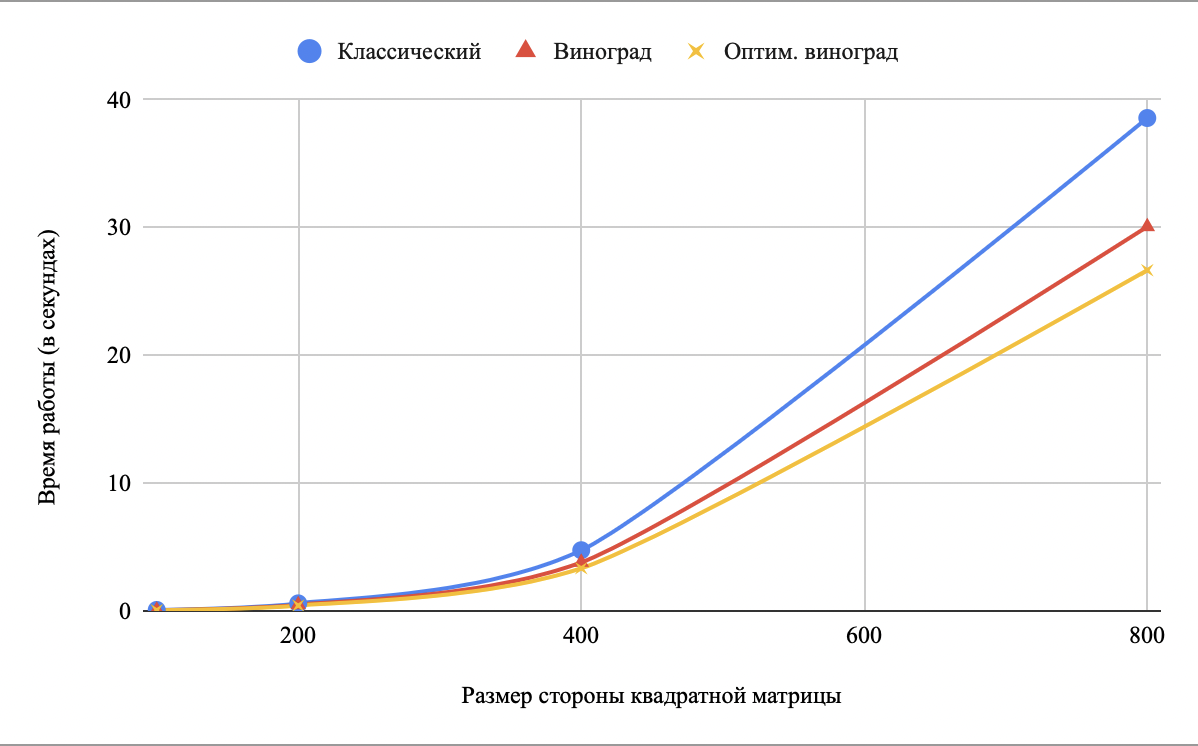
\includegraphics[scale=0.7]{plot_best.png}
    \caption{Зависимость времени выполнения алгоритмов от четного размера стороны квадратной матрицы}
    \label{img:plot_best}
\end{figure}

\begin{table}[p]
    \caption{\centering Время выполнения реализаций алгоритмов (в секундах) при нечетном размере матрицы}
    \centering
    \begin{tabular}{|c|c|c|c|}
    \hline
    Размер & К       & В      & ОВ     \\ \hline
    101    & 0.0741E & 0.0616 & 0.0551 \\ \hline
    201    & 0.590   & 0.475  & 0.429  \\ \hline
    401    & 4,7312  & 3,7858 & 3,3499 \\ \hline
    801    & 38,591  & 30,11  & 26,655 \\ \hline
    \end{tabular}
    \label{tab:time_worst}
\end{table}

\begin{figure}
    \centering
    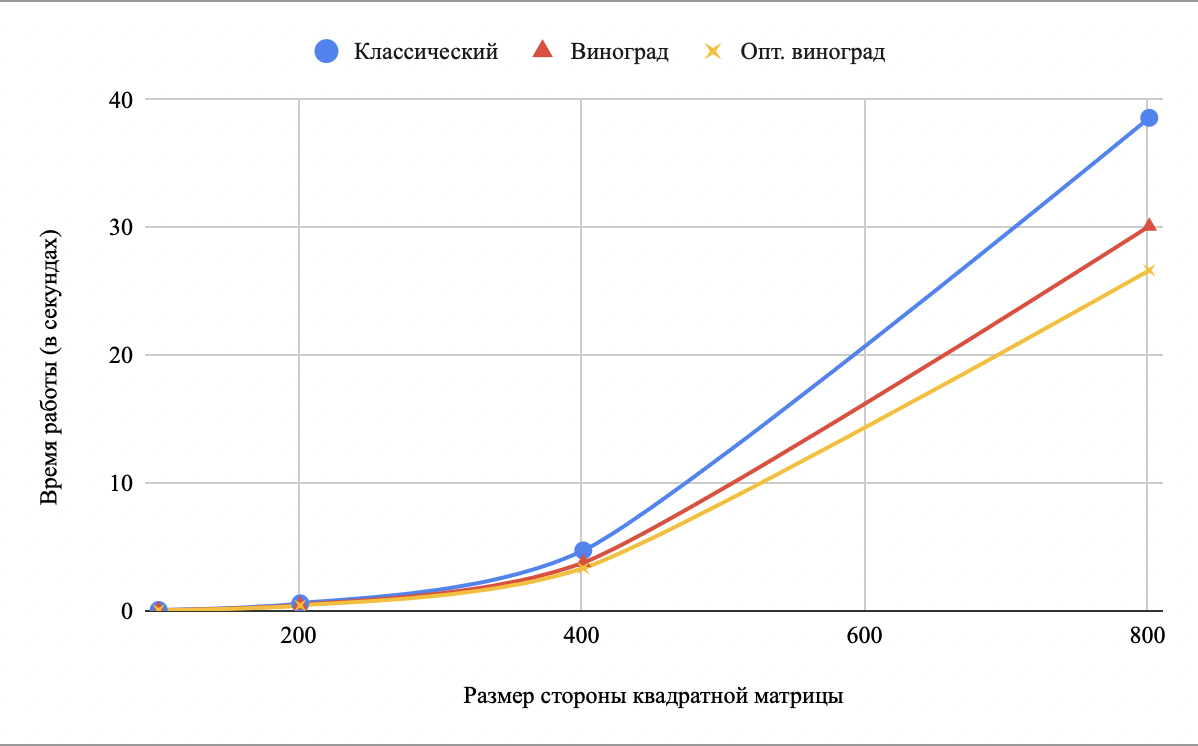
\includegraphics[scale=0.7]{plot_worst.png}
    \caption{Зависимость времени выполнения алгоритмов от нечетного размера стороны квадратной матрицы}
    \label{img:plot_worst}
\end{figure}

\subsection{Вывод}

Время работы реализации алгоритма Копперсмита–Винограда быстрее классического алгоритма умножения матриц примерно на 25-30\% быстрее. В то же время оптимизированный алгоритм Копперсмита–Винограда быстрее оригинального на 10-15\%. Таким образом на матрицах значительного размера (больше 200) следует использовать алгоритм Копперсмита–Винограда, так как он значительно быстрее (таблица \ref{tab:time_best}). 

Не смотря на то, что в аналитической части сложность алгоритма Винограда и оптимизированного Винограда больше, эти алгоритмы работают быстрее, так как в алгоритмах Винограда и оптимизированного Винограда используются выражения, которые предварительно обрабатываются, и это позволяет уменьшить количество умножений, но количество сложений увеличивается, но так как на реальных машинах операция сложения работает быстрее, то и сам алгоритм отрабатывает быстрее стандартного.

\anonsection{Заключение}

В ходе выполнения работы была достигнута цель выполнены все поставленные задачи:

\begin{itemize}
    \item рассчитать трудоемкость алгоритмов умножения матриц;
    \item реализовать классический алгоритм умножения матриц;
    \item реализовать алгоритм Копперсмита — Винограда;
    \item реализовать улучшенный Алгоритм Копперсмита — Винограда;
    \item сравнить их временные характеристики экспериментально;
    \item на основании проделанной работы сделать выводы.
\end{itemize}

Экспериментально были установлены различия в производительности различных алгоритмов умножения матриц. Оптимизированный алгоритм Копперсмита–Винограда имеет меньшую сложность, нежели оригинальный алгоритм умножения матриц Винограда. Так при размерах матриц $800 \times 800$ классический алгоритм отстает от алгоритма Копперсмита-Винограда на 45\%.

\anonsection{Литература}

\begin{enumerate}
    \item Ульянов М. В. Ресурсно-эффективные компьютерные алгоритмы. Разработка и Анализ. - Наука Физматлит, 2007. - 376.
    \item Блэнди Дж., Орендорф Дж. Программирование на языке Rust = Programming Rust. — ДМК Пресс, 2018. — 550 с. — ISBN 978-5-97060-236-2.
    \item LPDDR4 [Электронный ресурс] \url{https://ru.wikipedia.org/wiki/LPDDR#LPDDR4} (дата обращения: \today)
    \item Criterion.rs - Statistics-driven benchmarking library for Rust [Электронный ресурс] \url{https://github.com/bheisler/criterion.rs} (дата обращения: \today)
\end{enumerate}

\end{document}
